% SPDX-License-Identifier: GPL-2.0-or-later

% Copyright (C) 2020 Olivier Dion <olivier.dion@polymtl.ca>


\documentclass[12pt,letterpaper]{report}

\usepackage[letterpaper, top=0.5in]{geometry}
\usepackage{titlesec}
\usepackage{tocloft}
\usepackage{enumerate}
\usepackage[obeyspaces]{url}
\usepackage{algpseudocode}
\usepackage{graphicx}
\usepackage[utf8]{inputenc}
\usepackage{amsmath}
\usepackage{amssymb}
\usepackage[french]{babel}
\usepackage{pdfpages}
\graphicspath{ {.} }

\def\title{INF3710 - Fichiers et Bases de données}
\def\tpnumber{1}

\renewcommand{\b}[1]{\textbf{#1}}
\renewcommand{\i}[1]{\textit{#1}}
\newcommand{\var}[1]{\texttt{#1}}
\newcommand{\file}[1]{\path{#1}}
\newcommand{\vhdl}[1]{\mintinline{vhdl}{#1}}

\titleformat{\chapter}{\bf\huge}{\thechapter.}{20pt}{\bf\huge}
\renewcommand*\contentsname{Table of Contents}

\renewcommand{\cftchapleader}{\cftdotfill{\cftdotsep}}
\renewcommand\cftchapfont{\Large\bfseries}
\renewcommand\cftchappagefont{\Large\bfseries}
\renewcommand\cftchapafterpnum{\par\addvspace{6pt}}

\renewcommand{\cftsecleader}{\cftdotfill{\cftdotsep}}
\renewcommand\cftsecfont{\large}
\renewcommand\cftsecpagefont{\large}
\renewcommand\cftsecafterpnum{\par\addvspace{6pt}}

\setlength{\parskip}{0.5em}

\begin{document}


\begin{titlepage}
  Prof. Amal Zouaq (Hiver 2020)
  \vfill
  \vskip 2cm
  \begin{center}
    
\includegraphics{polymtl}
    \vskip 2cm
    \title
    \vskip 1cm
    Hiver 2020
    \vskip 1cm
    TP No. \tpnumber
    \vskip 1cm
    Groupe 2
    \vskip 1cm
    1893306 - Karl Dunkelmann
    1927844 - Olivier Dion

    \vskip 1cm

    Soumis à :

    \vskip 1cm

    \today

  \vskip 0pt plus 1filll
  
\end{center}
\vfill

\end{titlepage}

%%% Local Variables:
%%% mode: latex
%%% TeX-master: "lab"
%%% End:


\newpage

\begin{figure}[h]
  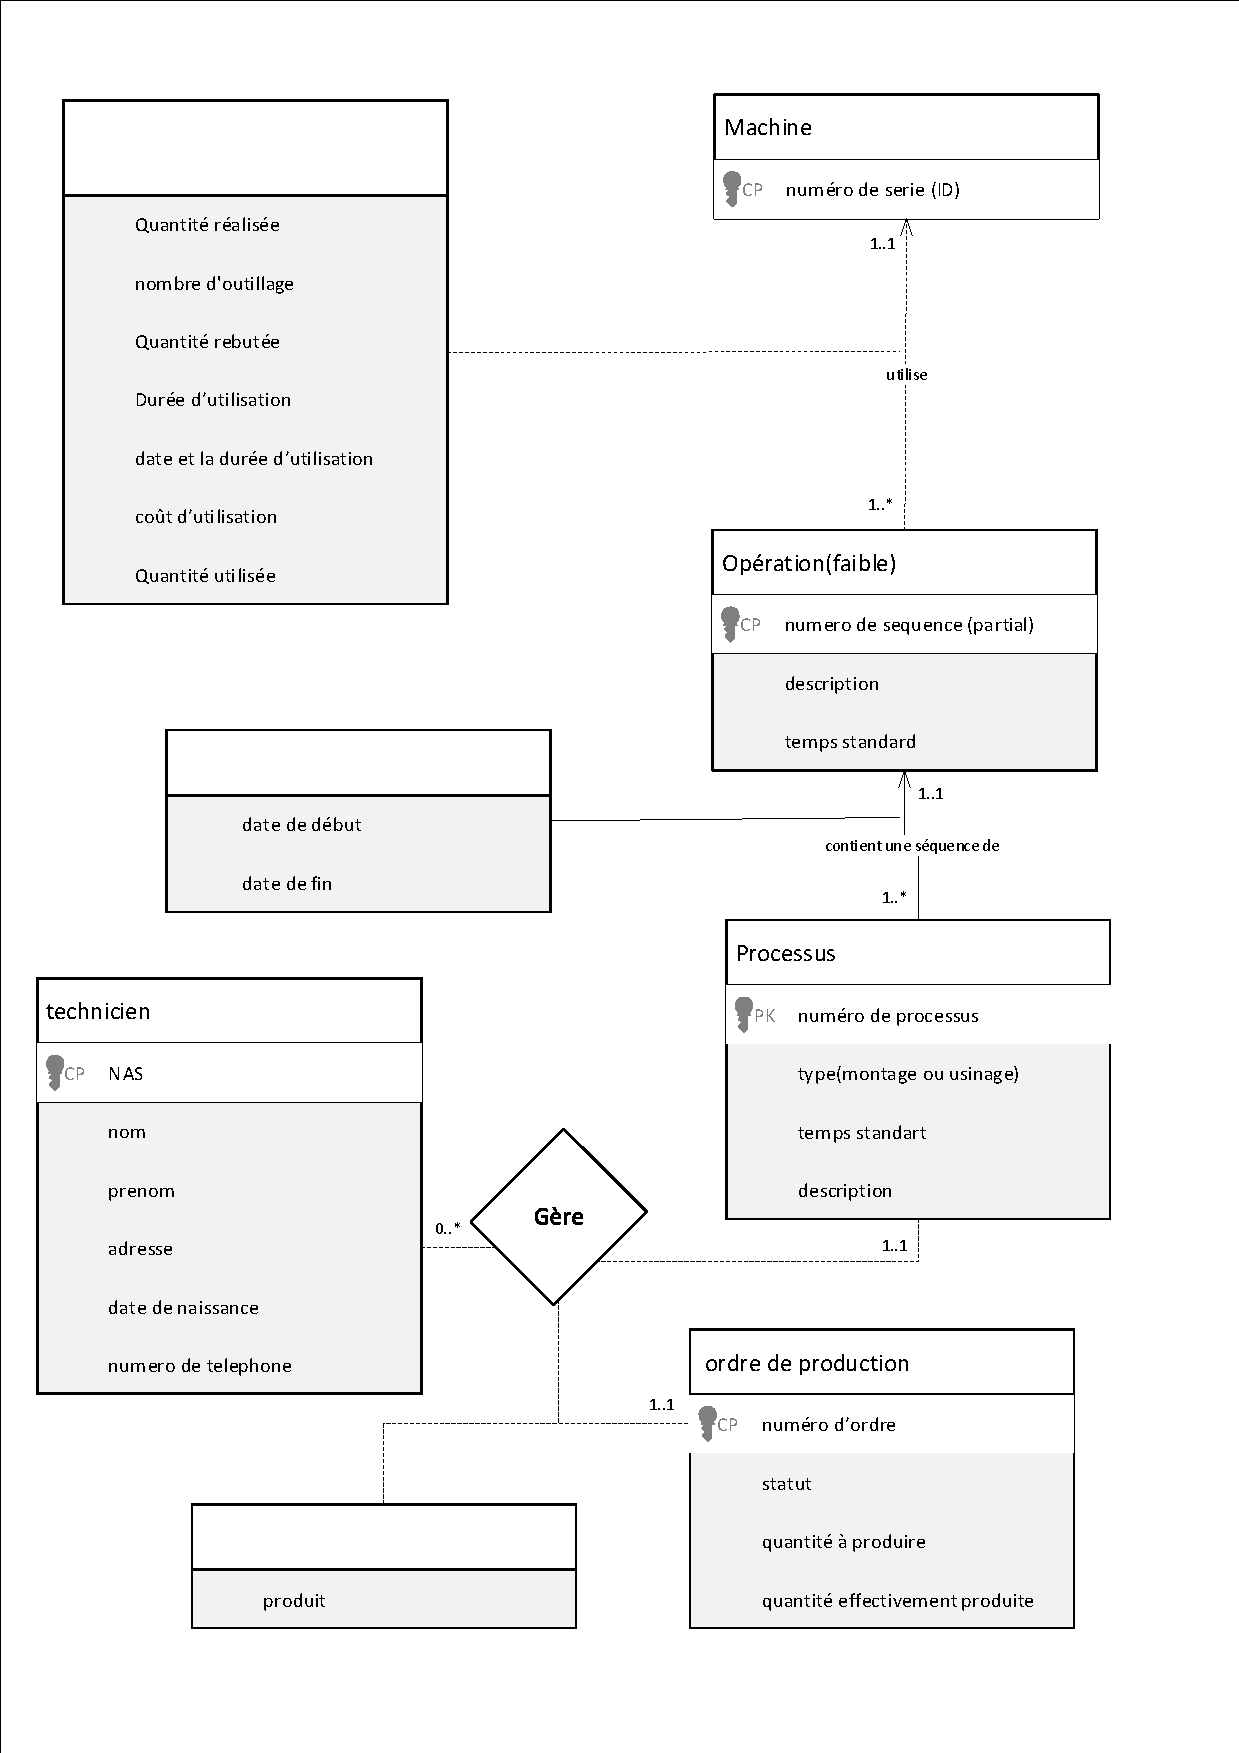
\includepdf[scale=0.85,pages=1]{graph.pdf}
\end{figure}

\newpage

\chapter{Commentaire}

\section{Relation technicien, processus et ordres de production}

Les relations entre les entités \b{technicien}, \b{processus} et
\b{ordres de production} se lisent comme suit:

Un technicien gère 0 à plusieurs processus selon un ordre et un
processus est géré par un seul technicien selon un ordre.  Il s'agit
de relations non identifiantes.  Ces relations possèdent comme
attribut le produit à produire.


\section{Relation processus et opération}
La relation entre \b{processus} et \b{opération} se lit comme suit:

Un processus est contient (est composé de) une séquence d'opérations
et une opération appartient à un seul processus.  Cette relation
possède une date de début et de fin comme attributs.  Il s'agit d'une
relation identifiante, car une opération est une entité faible.


\section{Relation opération et machine}
La relation entre une \b{opération} et une \b{machine} se lit comme suit:

Une opération utilise une ou plusieurs machines, et une machine peut
être utilisée que par une opération à la fois.  Cette utilisation est
une relation non identifiante qui possède de nombreux attributs, tels
que les outillages utilisés, le coût d'utilisation, etc.




\end{document}


%%% Local Variables:
%%% mode: latex
%%% TeX-master: t
%%% End:
